%\documentclass{beamer}
\documentclass[handout]{beamer}
%\usetheme{boxes} 
\usetheme{default}

%math fonts
%\renewcommand\mathfamilydefault{\rmdefault}

%page numbers
\setbeamertemplate{footline}[page number]
\setbeamertemplate{section in head/foot}{\hfill\insertsectionheadnumber.~\insertsectionhead}
\setbeamertemplate{section in head/foot shaded}{\color{structure!50}\hfill\insertsectionheadnumber.~\insertsectionhead}
\setbeamertemplate{section in toc}{\inserttocsectionnumber.~\inserttocsection}

\setbeamercovered{invisible}
\setbeamertemplate{navigation symbols}{} 
\usepackage{mathtools}
\usepackage{graphicx}
\usepackage{amsmath}
\usepackage{epstopdf}
\usepackage{color}
\usepackage{subfig}
\usepackage{hyperref}
\usepackage{multimedia}


\title[Probabilistic Modelling for Table Tennis]{A New Performance Criterion in Robotic Table Tennis}
\author{Okan Ko\c{c}}
\institute[IAS]
{
MPI for Intelligent Systems, T\"ubingen \\
Robot Learning Lab \\
\medskip
{\emph{okan.koc@tuebingen.mpg.de}}
}
\date{\today}

% custom commands
\newcommand{\boldvec}[1]{\boldsymbol{\mathrm{#1}}}
\let\vec\boldvec
\newcommand\at[2]{\left.#1\right|_{#2}} % the at differential sign
\newcommand\scalemath[2]{\scalebox{#1}{\mbox{\ensuremath{\displaystyle #2}}}} % scaling matrices

% % % % % CUSTOM COMMANDS GO HERE
% % % % % % % % Notation for robot % % % % % % %
\newcommand{\todo}{\textcolor{red}{TODO}} % TODO!
\newcommand{\kin}{\mathcal{K}} % used to denote forward kinematics
\newcommand{\invKin}{\mathcal{K}^{-1}} % used to denote inverse kinematics
\newcommand{\jacobian}{\vec{J}(\joint)} % jacobian

\newcommand{\joint}{\vec{q}} % used to denote robot state in joint space
\newcommand{\state}{\vec{y}} % denotes the generalized coordinates - joint angles and angular velocities
\newcommand{\error}{\vec{e}} % difference between state and reference
\newcommand{\traj}{\vec{r}} % used to denote the points on the trajectory to be tracked

\newcommand{\dynamics}{\vec{f}}
\newcommand{\dynamicsNominal}{\dynamics_{\mathrm{nom}}}
\newcommand{\dist}{\vec{\epsilon}} % denotes the disturbances acting on the rigid body dynamics
\newcommand{\sysInput}{\vec{u}} % used to denote the system inputs
\newcommand{\trjInput}{\sysInput_{\mathrm{IDM}}} % denotes the inputs on the trajectory (calculated using IDM)

\newcommand{\policy}{\vec{\pi}}
\newcommand{\ValueFunction}{J}
\newcommand{\episode}{k} % used for episode number
\newcommand{\totalTime}{T} % total time duration 
\newcommand{\numSteps}{N} % total number of time steps
\newcommand{\threshold}{\epsilon}
\newcommand{\alg}{\emph{ptt}} % probabilistic table tennis
\newcommand{\dataset}{\mathcal{D}}

% % % % % % % % Table tennis notation % % % % % %
\newcommand{\ballFull}{\vec{x}_{B}} % ball cartesian state
\newcommand{\ball}{\vec{b}} % ball positions
\newcommand{\ballRadius}{r_B}
\newcommand{\ballVel}{v} 
\newcommand{\ballDynamics}{\vec{F}} % ball dynamics
\newcommand{\drag}{C} % drag
\newcommand{\gravity}{g}
\newcommand{\bounce}{\vec{E}} 
\newcommand{\contact}{\vec{C}} % contact model
\newcommand{\racket}{\vec{r}} % racket positions
\newcommand{\racketRadius}{r_R} % racket radius
\newcommand{\orient}{\vec{o}} % racket orientations
\newcommand{\normal}{\vec{n}} % racket normal
\newcommand{\robot}{\vec{x}_{R}} % racket state involving pos,vel and orient
\newcommand{\stabilityRegion}{\mathcal{S}} % stability region in ball phase space
\newcommand{\court}{\mathcal{T}} % opponents court
\newcommand{\net}{\mathcal{N}} % net
\newcommand{\wall}{\mathcal{W}} % wall

% % % % % % % % Probability notation % % % % % % %
\newcommand{\prob}{\mathbb{P}} % probability
\newcommand{\landTime}{\tau} % random variable
\newcommand{\landEvent}{\mathcal{L}} % land on table
\newcommand{\landDist}{p(\tau)} % distribution of landing time
\newcommand{\hitTime}{\nu} % hitting time
\newcommand{\hitEvent}{\mathcal{H}}
\newcommand{\hitDist}{p(\nu)} % distribution of hitting time
\newcommand{\KL}{D_{\mathrm{KL}}}

% Set the paths where all figures are taken from:
\graphicspath{{Pictures/}}
\mathtoolsset{showonlyrefs} 
\newcommand{\includesvg}[1]{%
% \executeiffilenewer{#1.svg}{#1.pdf}%
% {inkscape -z -D --file=#1.svg %
% --export-pdf=#1.pdf --export-latex}%
 \input{#1.pdf_tex}%
}

\begin{document}
%
\begin{frame}
\titlepage
\end{frame}
%
\begin{frame}
\frametitle{Table of Contents}
\tableofcontents
\end{frame}
%
\section{Last Project}
%
\begin{frame}{Table Tennis Setup}
\begin{itemize}
\item Ballgun facing Barrett WAM, his deadly opponent.
\end{itemize}
\begin{figure}[b!]
\center
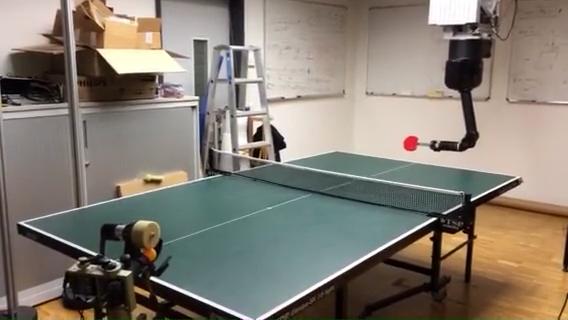
\includegraphics[scale=0.4]{robot1.png}			
\label{robot}
\caption{Ballgun faces his deadly opponent!}
\end{figure}
\end{frame}
%
\begin{frame}{Optimizing Robot Striking Movement Primitives with ILC}
\begin{itemize}
\item Tracking a rhythmic DMP with ILC.
\item Future work will focus on generalizing ILC between different trajectories.
\end{itemize}
\begin{figure}[ht]
\centering
\subfloat{%
\includegraphics[width=0.6\linewidth]{actualResult.eps}}
\subfloat{%
\movie[externalviewer]{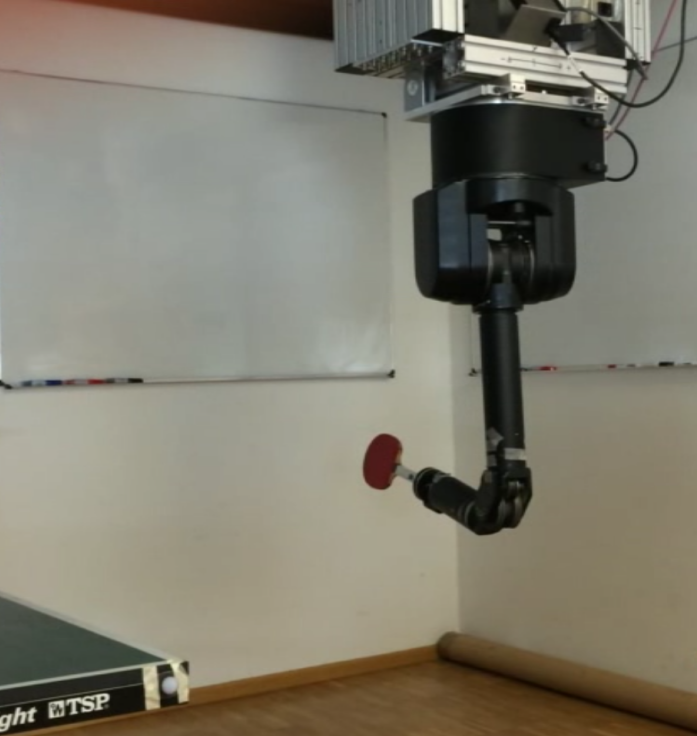
\includegraphics[scale=0.3]{ilcBarrettWAM.png}}{ilcBarrettWAM.mp4}}
%\caption{DMPs are nice!} 
\label{Robot experiment} 
\end{figure}
% put a video here and Humanoids'15 heading
% talk about generalizing ILC to table tennis trajectories
\end{frame}
%
\section{Motivation}
%
\begin{frame}{Motivation}
\begin{itemize}
\item Trajectory generation in robotic table tennis does not incorporate uncertainty, i.e. no probabilistic modelling.
\item Virtual Hitting Plane (VHP) used to generate trajectories.
\end{itemize}
\begin{figure}[t!]
\center
%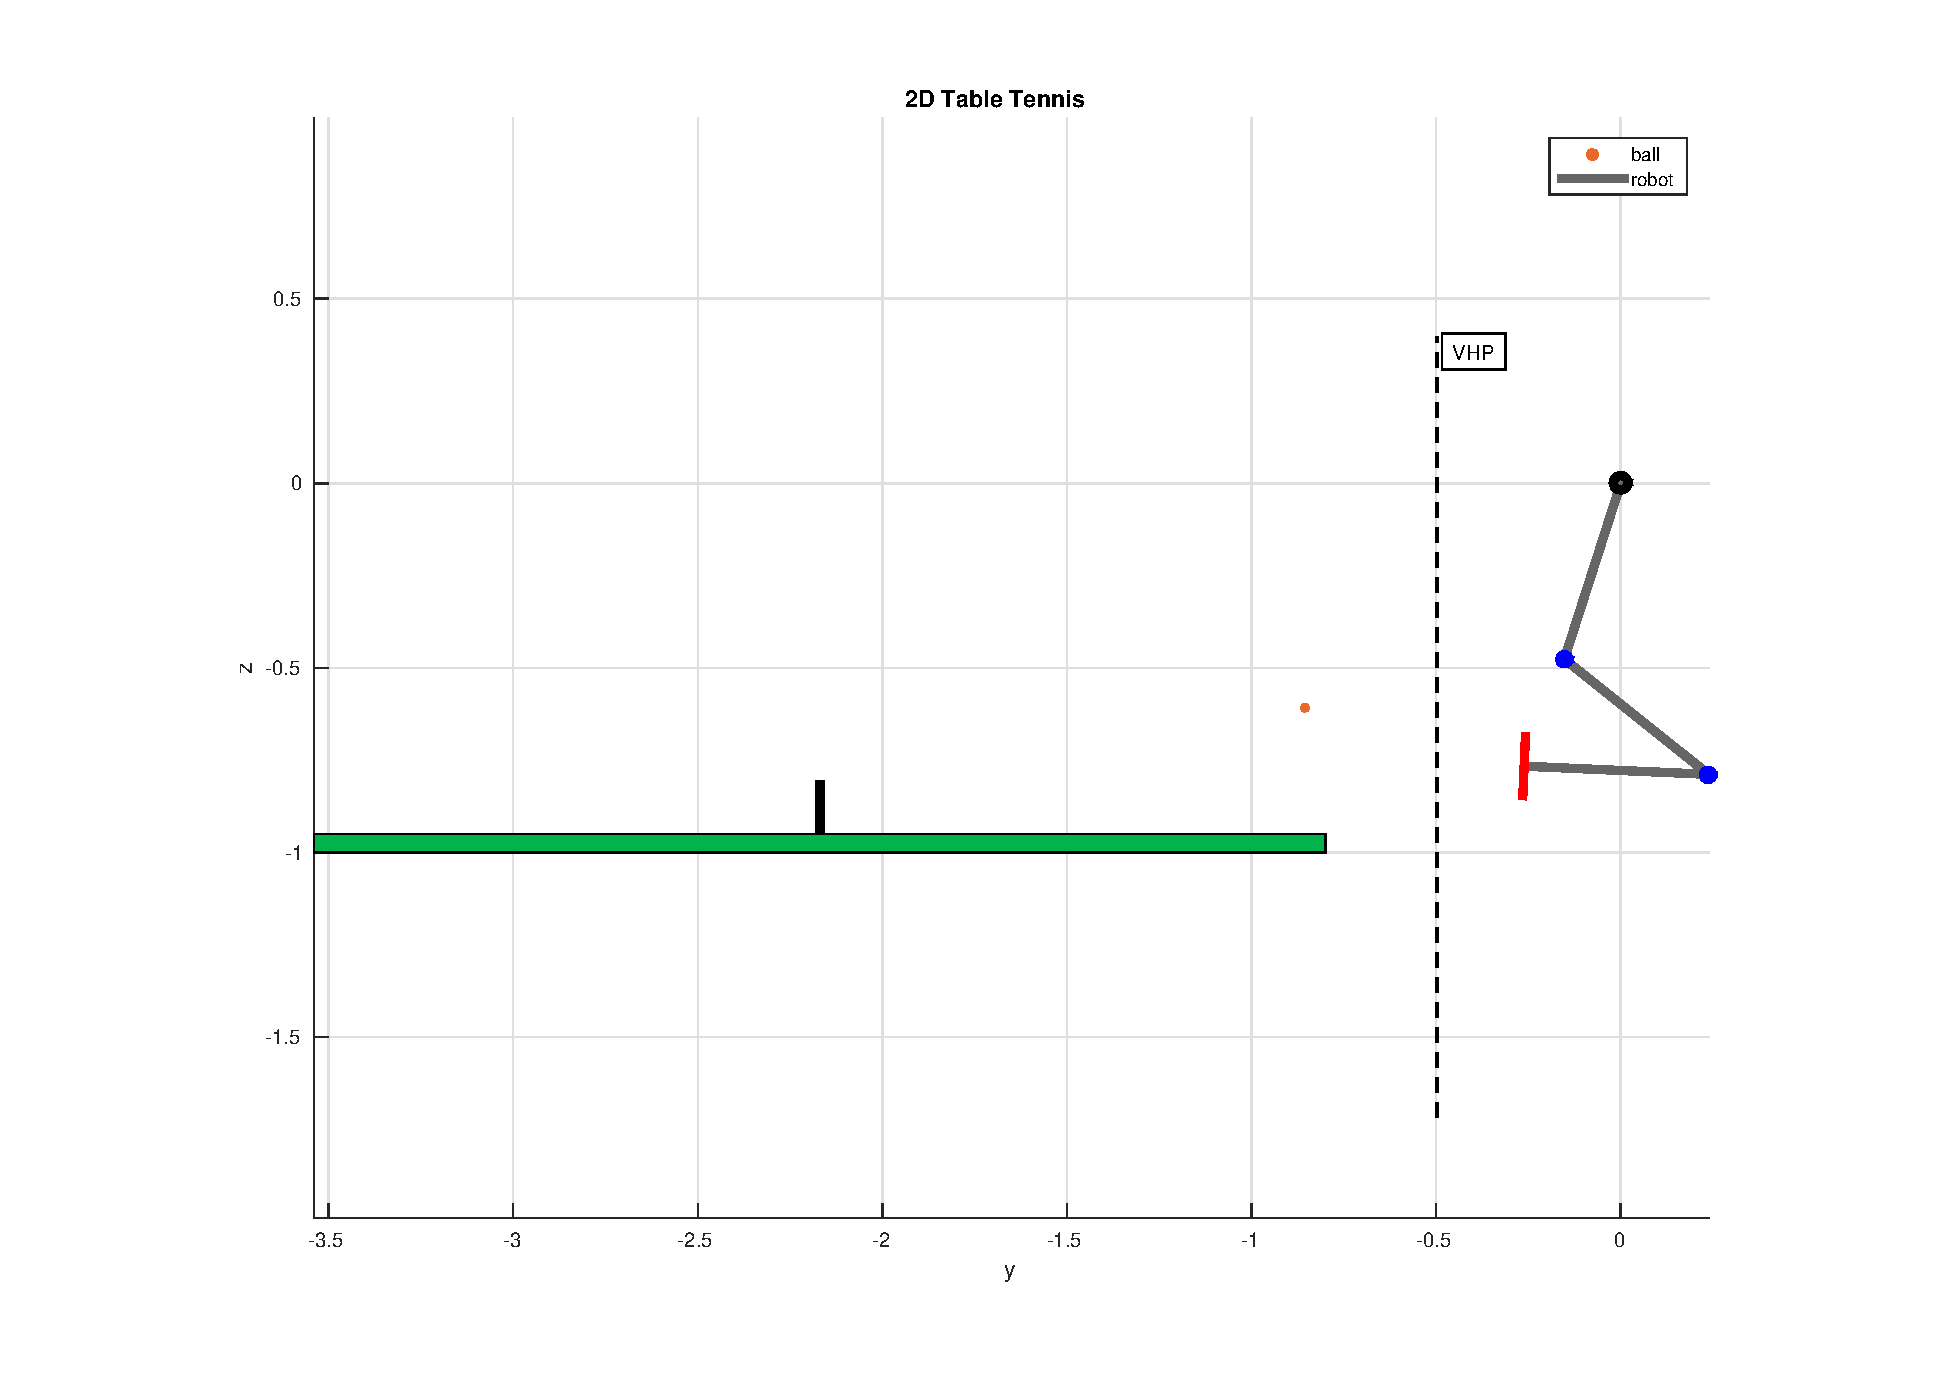
\includegraphics[scale=0.20]{tableTennis2D.eps}	
\movie[externalviewer]{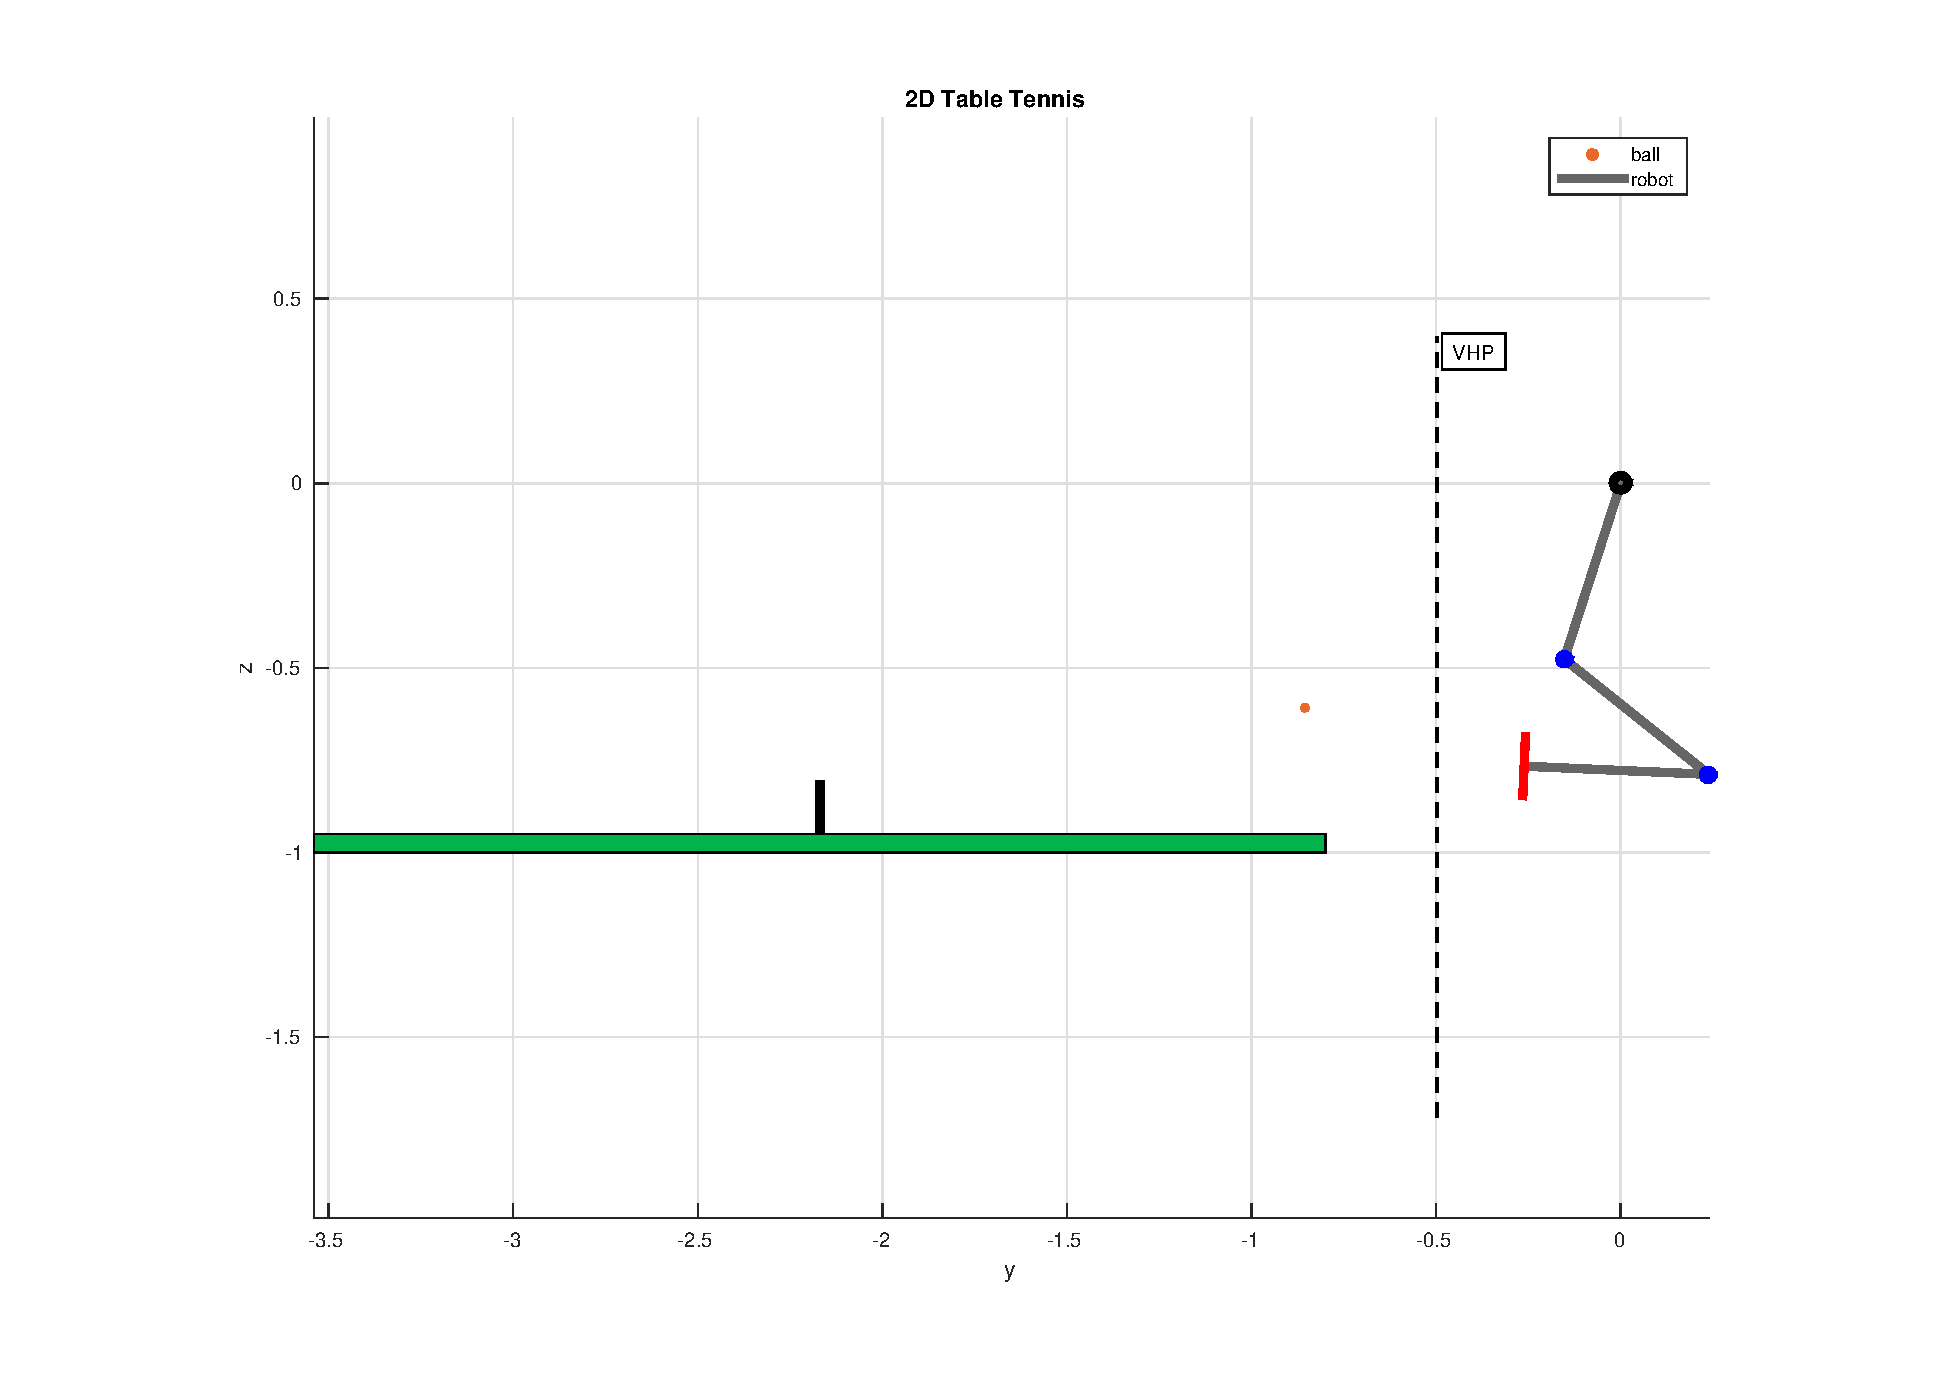
\includegraphics[scale=0.2]{tableTennis2D.eps}}{out.ogv}		
\caption{2D Table Tennis with VHP}
\label{robot1}
\end{figure}
\end{frame}
%
\begin{frame}{Motivation}
\begin{itemize}
\item Fix a hitting plane, use flight and rebound models to predict the intersection point. 
\item Use inverse kinematics to construct the reference trajectory in joint space.
\end{itemize}
\begin{figure}[t!]
\center
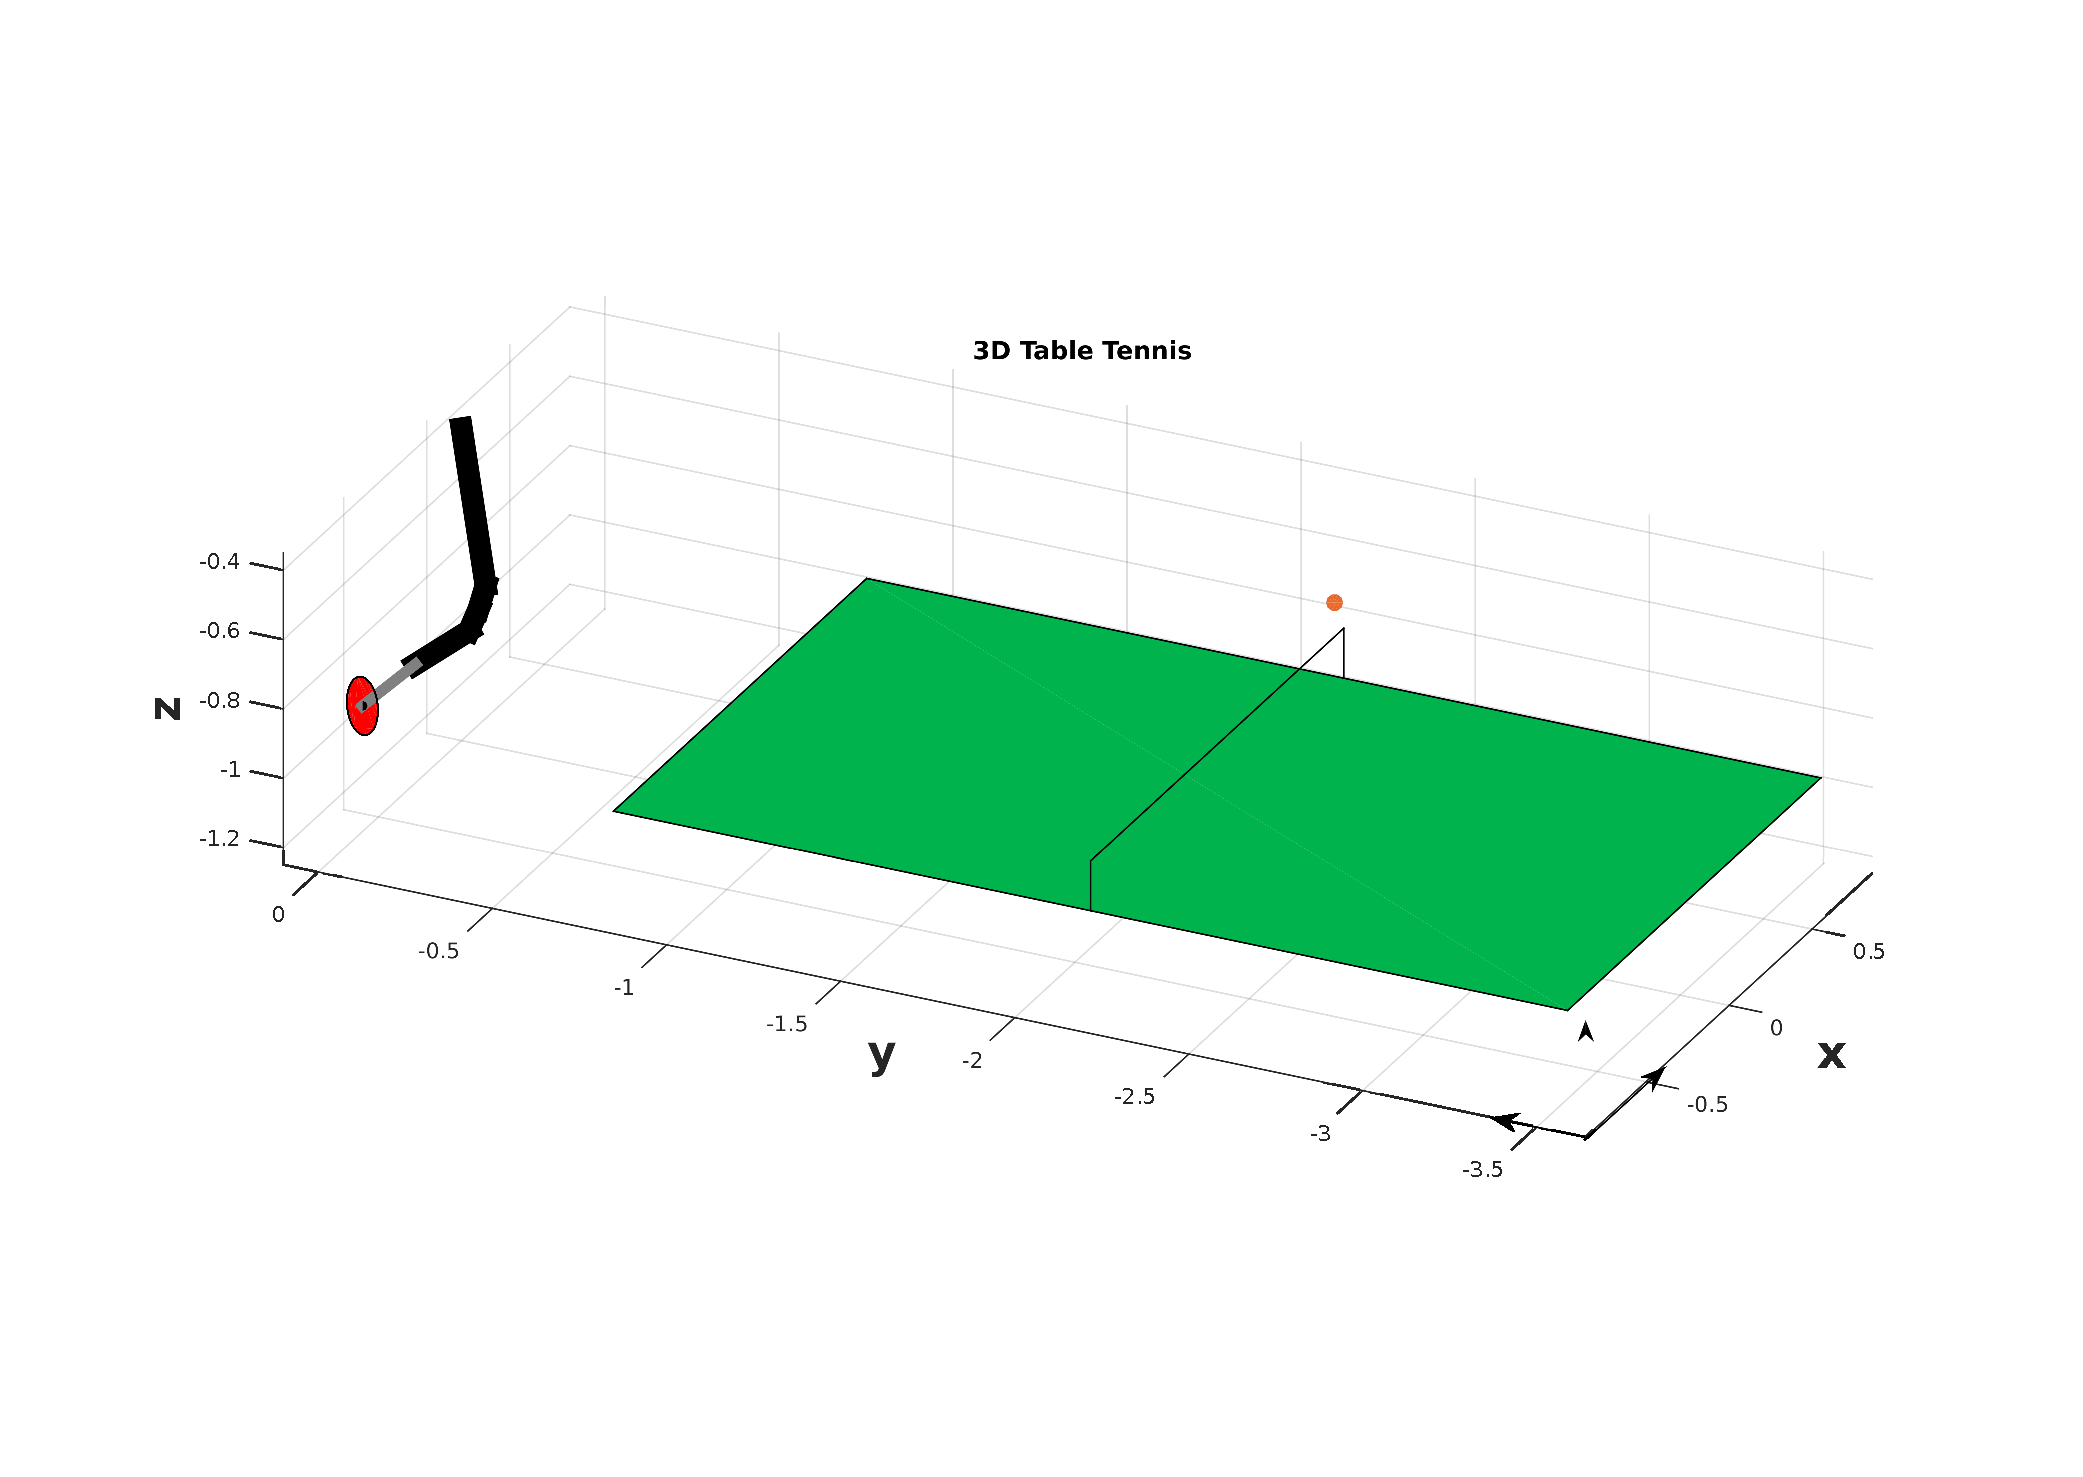
\includegraphics[scale=0.30]{tableTennis3D.eps}			
\caption{3D Table Tennis}
\label{robot2}
\end{figure}
\end{frame}
%
\begin{frame}{Research Question}
\begin{itemize}
\item Find out a (optimal,robust) racket trajectory that returns the balls with a high probability to the opponent's court.
\end{itemize}
\begin{figure}[t!]
\centering
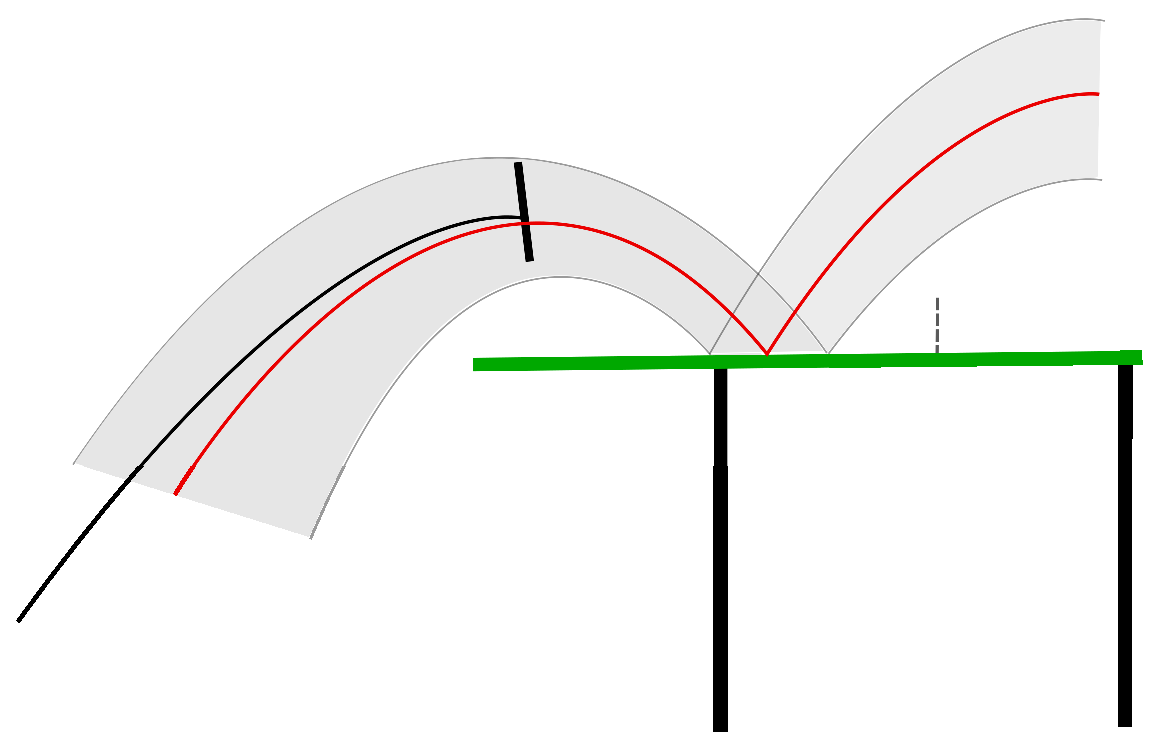
\includegraphics[scale=0.4]{drawing.eps}			
\caption{Illustrating the main idea. From the racket's point of view, the ball motion is a stochastic process.}
\label{mainIdea}
% from the ball's point of view, a racket trajectory in table tennis has a certain probability of hitting the ball and a significantly smaller probability of landing it (legally) on the opponents court. From the racket's point of view, the ball motion is a certain stochastic process and it should be intercepted such that the marginal probability distribution at hitting time is transformed at landing time to a desired marginal distribution.
\end{figure}
\end{frame}
%
\section{Methodology}
%
\begin{frame}{Problem Setting}
\begin{figure}[t!]
\centering
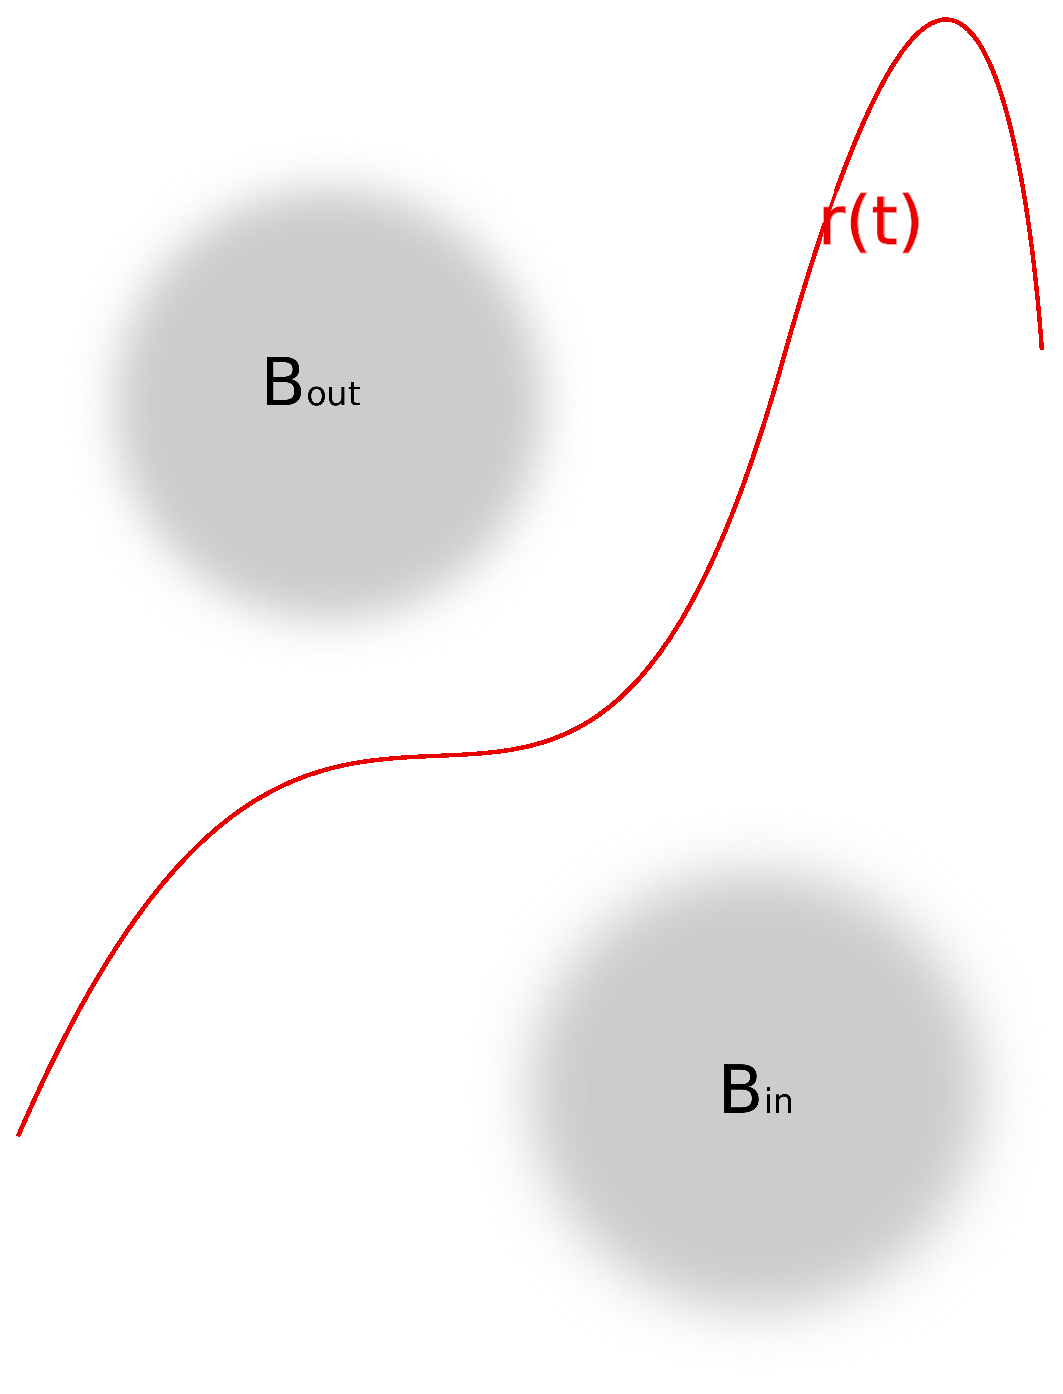
\includegraphics[scale=0.3]{drawingBallsEye.eps}			
\caption{Illustrating the main idea. From the ball's point of view, a racket trajectory $r(t)$ has a certain probability of hitting the ball and a significantly smaller probability of landing it on the opponents court.}
\label{mainIdea2}
\end{figure}
\end{frame}
%
\begin{frame}{Method}
\begin{itemize}
\item \emph{Free-time} optimal control problem
%
\begin{align}
\min_{\sysInput,T} & \int\limits_{0}^{T}\sysInput(t)^{\mathrm{T}}\vec{R}\sysInput(t) + \KL(p(b_x,b_y|\landEvent)||\mathcal{U}(\court)), \\
& \textrm{s.t. } \ddot{\joint}(t) = \sysInput(t),
\label{costFnc1}
\end{align}
%
\item $T$ is the final time of the racket trajectory 
%
\begin{align}
\big(\racket(t),\orient(t)\big) &= \kin(\joint(t)),
\end{align}
\end{itemize}
\end{frame}
%
%
\begin{frame}{KL-divergence}
\begin{itemize}
%
\item $\KL(p(b_x,b_y|\landEvent)|\mathcal{U}(\court))$ maximizes the probability of landing on the opponents court while ensuring unpredictability.
\item Difficult to compute, and optimize!
\end{itemize}
\begin{figure}[t!]
\center
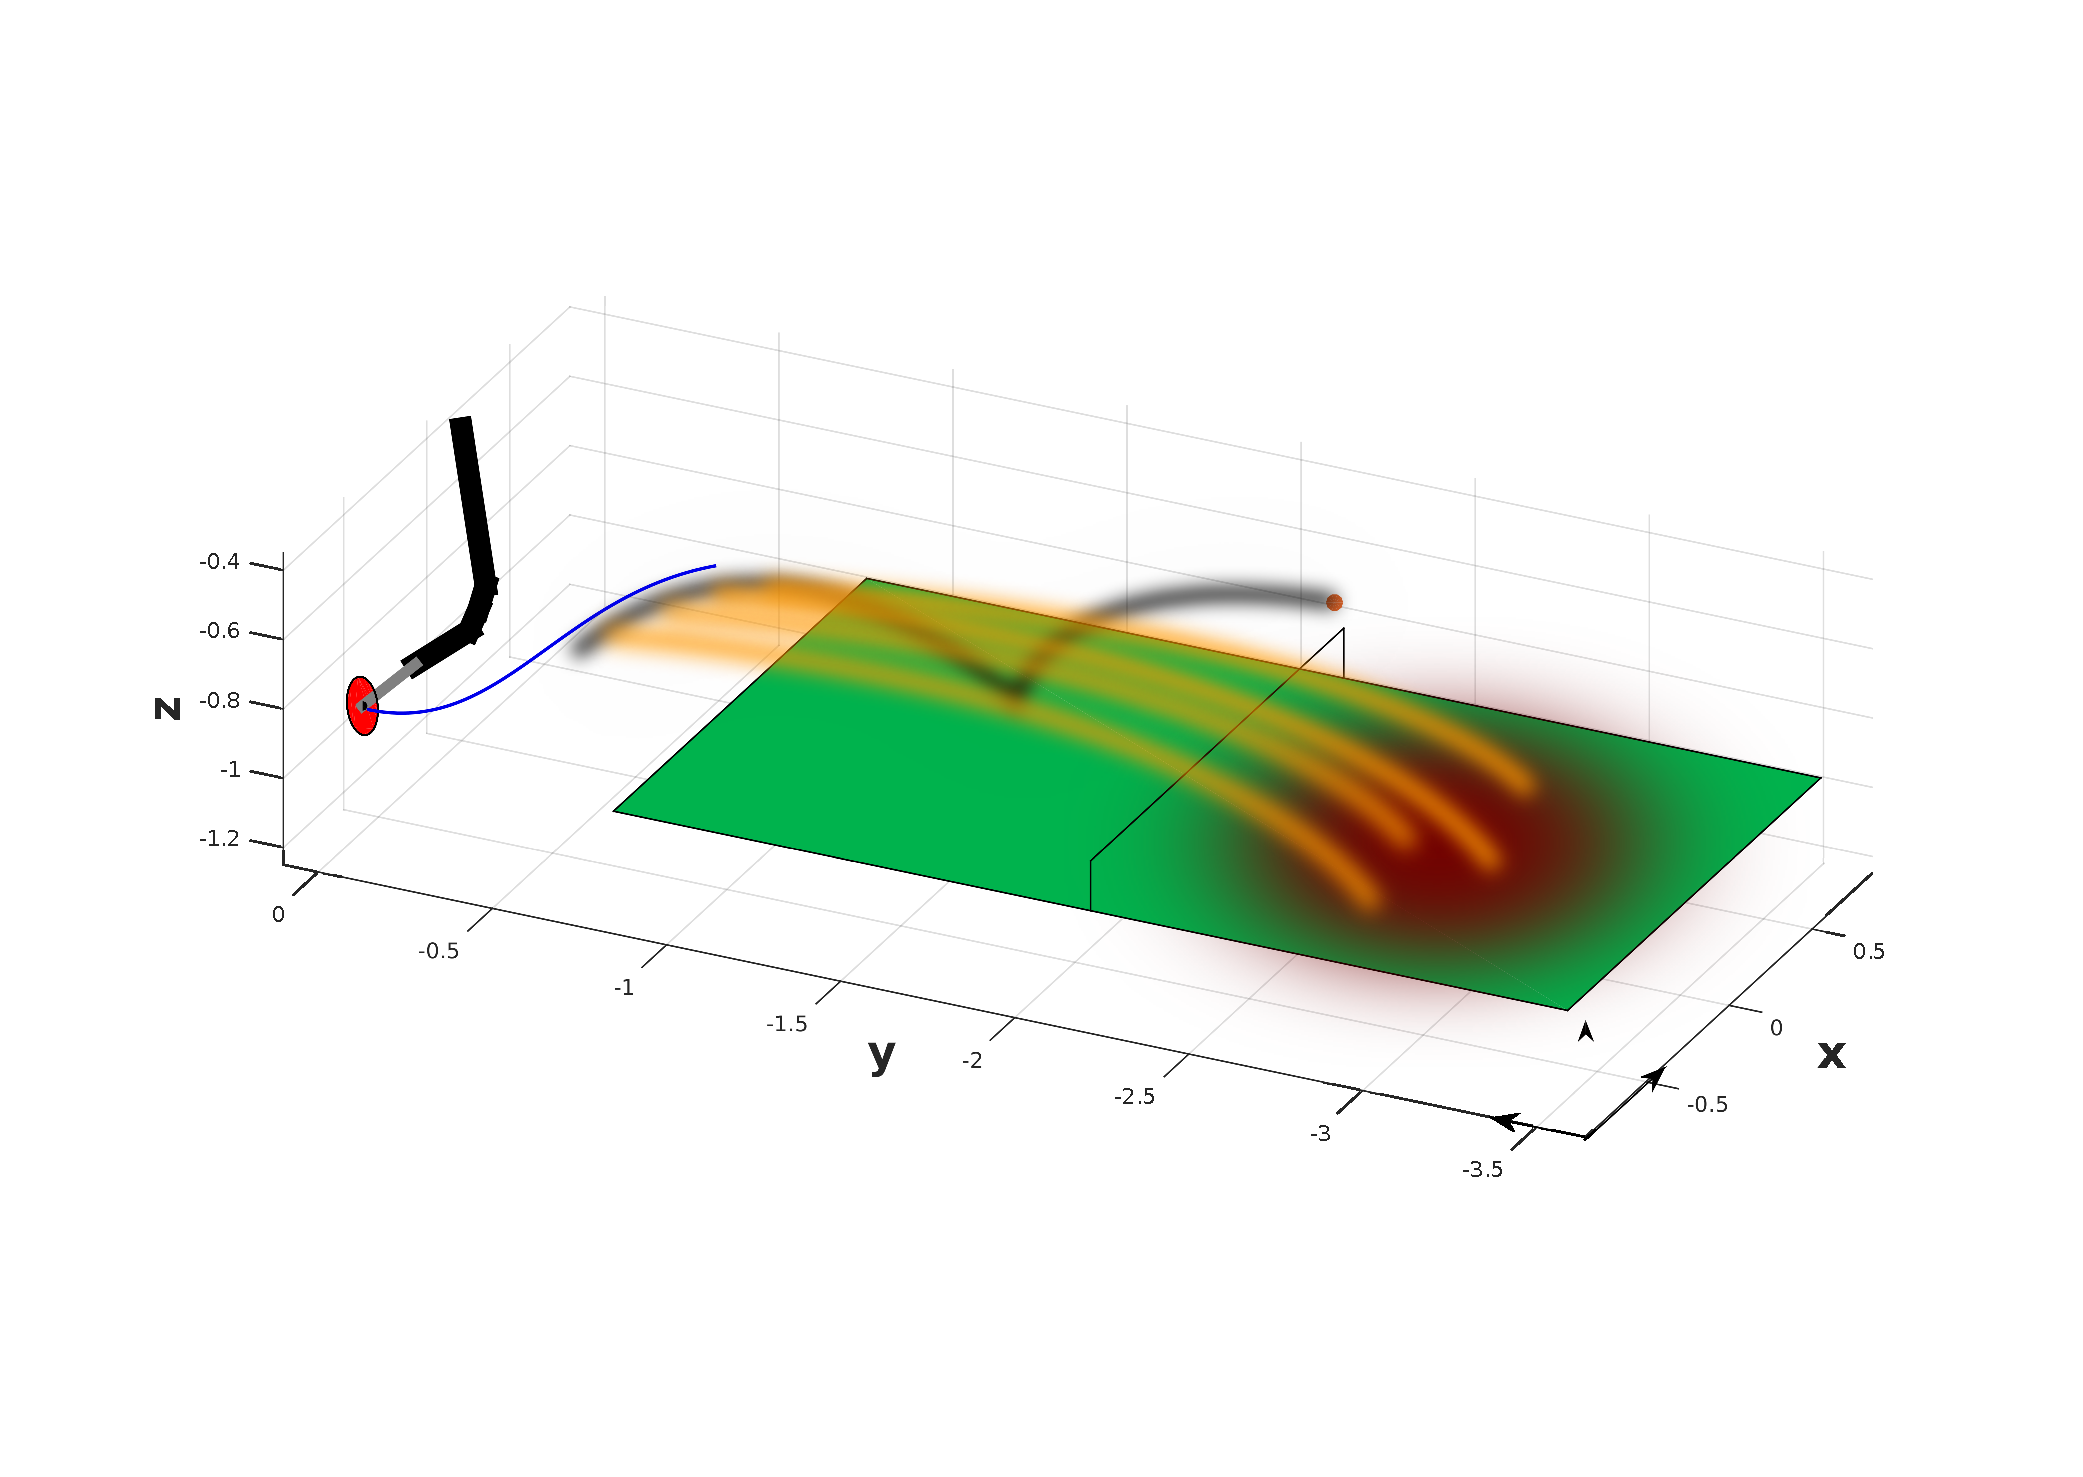
\includegraphics[scale=0.3]{tableTennis3DwithUncertainty.eps}			
\caption{3D Table Tennis}
\end{figure}
\end{frame}
%
\section{Algorithm}
%
\begin{frame}{Algorithm}
\begin{itemize}
\item Initialize by solving maximum principle with transversality conditions, e.g.
%
\begin{align}
\min_{\sysInput,T} & \int\limits_{0}^{T}\sysInput(t)^{\mathrm{T}}\vec{R}\sysInput(t) \\
\textrm{s.t. } & \ddot{\joint}(t) = \sysInput(t), \\
& \kin(\joint(t)) = \ball(t), \\
& \jacobian \dot{\joint}(t) = -\dot{\ball}(t).
\label{costFnc2}
\end{align}
%
\item Optimize further by simulating: sampling from an initial distribution $\ball_t \sim \mathcal{N}(\mu(t),\Sigma(t))$
\end{itemize}
\begin{align}
p(b_x,b_y|\landEvent) = \int_{\landTime = 0}^{\infty} p_{\landTime}(b_x,b_y|\landEvent,\landTime)\landDist \textrm{d}\landTime
\label{marginalProcess} \\
\end{align}
% put the sampling based algorithm here
\end{frame}
%
\begin{frame}{Future Work}
\begin{itemize}
\item (Approximate) closed form gradients ?
\item Solve the optimization problem fast in real time.
\item Compensate for tracking errors with ILC.
\end{itemize}
% show simulation results in 2d and 3d table tennis
% real robot results 
\end{frame}
%
\begin{frame}{Conclusion}
\begin{itemize}
\item Thank you for listening!
\end{itemize}
\end{frame}	
%
%\section{References}
%\begin{frame}[allowframebreaks]{References}
%\def\newblock{\hskip .11em plus .33em minus .07em}
%\bibliographystyle{alpha}
%\bibliography{myReferences} % file name of the bibtex
%\end{frame}
%

%
% End of slides
\end{document} 